\documentclass[11pt]{article}
\usepackage[letterpaper,margin=1.05in]{geometry}
\usepackage[T1]{fontenc}
\usepackage{lmodern}
\usepackage{amsmath,amssymb,amsthm}
\usepackage{booktabs}
\usepackage{microtype}
\usepackage{tabularx}
\usepackage{tikz}
\usepackage[colorlinks=true,linkcolor=blue!40!black,urlcolor=blue!40!black,citecolor=blue!40!black]{hyperref}
\hypersetup{pdftitle={Minimal Expansions Preserving Simple Random Walks},
  pdfsubject={Extremal faithful expansions of finite simple graphs},
  pdfkeywords={random walks, graph morphisms, vertex covers, lumpability}}
\usetikzlibrary{positioning}
\newtheorem{theorem}{Theorem}[section]
\newtheorem{lemma}[theorem]{Lemma}
\newtheorem{proposition}[theorem]{Proposition}
\newtheorem{corollary}[theorem]{Corollary}
\theoremstyle{definition}
\newtheorem{definition}[theorem]{Definition}
\newtheorem{example}[theorem]{Example}
\numberwithin{equation}{section}
\setlength{\emergencystretch}{2em}
\setlength{\parskip}{0pt}
\raggedbottom
\newcommand{\V}{V}
\newcommand{\E}{E}
\newcommand{\N}{N}
\newcommand{\Prob}{\mathbb P}
\title{Minimal Expansions Preserving Simple Random Walks}
\author{}
\date{October 6, 2026}

\begin{document}
\maketitle

\begin{abstract}
Let $G$ be a finite connected simple graph with at least two vertices.
A faithful expansion of $G$ is a connected simple graph $H$ equipped with
a surjection onto $G$ that sends simple random walk on $H$ to simple random
walk on $G$ for every initial state. We prove that the minimum order of a
nontrivial faithful expansion is $|\V(G)|+\tau(G)$, where $\tau(G)$ is the
vertex-cover number. Every such expansion has at least $2|\E(G)|$ edges,
and the two bounds are attained simultaneously. We characterize all
order-minimizing expansions and show that their number, up to isomorphism
over a fixed labeled base, is
$\sum_{S}2^{\beta(G[S])}$, where $S$ ranges over the minimum vertex covers
and $\beta$ denotes cycle rank. Consequences include an exact formula for
the cycle rank of an optimal expansion, preservation under time-dependent
replacement, and an exponential edge bound for nested strict expansions.
The arguments use classical degree conservation for harmonic morphisms.
The role of unit edge weights is demonstrated by a contrasting weighted
construction, and exhaustive finite checks accompany the proofs.
\end{abstract}

\medskip
\noindent\textbf{Keywords.} Simple random walk; harmonic morphism; vertex cover;
graph expansion; lumpability.

\section{Introduction}\label{sec:intro}

Suppose that the vertices of a graph represent observable states, and that
each state may be realized by several microscopic vertices. A natural
requirement on such a realization is that a simple random walker, observed
only through the original state labels, should retain its entire trajectory
law. This requirement permits substantial changes in the underlying graph:
for example, a four-cycle projects faithfully onto a three-vertex path by
identifying opposite vertices. The resulting extremal question is how few
vertices and edges a nontrivial realization can have.

For a graph $G$, let $\tau(G)$ be its vertex-cover number and $\alpha(G)$ its
independence number. We show that every nontrivial faithful expansion $H$
satisfies
\[
 |\V(H)|\ge |\V(G)|+\tau(G),\qquad
 |\E(H)|\ge 2|\E(G)|,
\]
with simultaneous equality attainable for every connected simple base.
An optimal construction takes two copies of $G$ and identifies the copies
of a maximum independent set. More generally, all order-minimizing
expansions arise from minimum vertex covers, with binary matching choices
on the edges induced by the cover. These choices yield an exact enumeration
over a fixed labeled base.

The probabilistic condition is a specialization of strong lumpability,
which requires a projected Markov chain to be Markov with the same transition
kernel for every initial distribution; see Geiger and Temmel~\cite{GT}.
For simple random walks on unweighted graphs, it is also the local-balance
condition for a nondegenerate harmonic morphism without contracted edges.
The corresponding degree theory and its composition properties are
classical; see Baker and Norine~\cite{BN}. The present manuscript gives a
self-contained extremal treatment of this setting. Historical priority of
the minimum-order formulation and its enumeration has not been established,
and no priority claim is made.

Section~\ref{sec:prelim} fixes the model.
Section~\ref{sec:minimum} proves the extremal bounds, and
Section~\ref{sec:classification} classifies their order-minimizing cases.
Section~\ref{sec:consequences} develops topological and temporal consequences.
Section~\ref{sec:weights} treats the weighted variant and the scope of the
observation model. Computational checks appear in Section~\ref{sec:checks}.

\section{Preliminaries and faithful expansions}\label{sec:prelim}

All graphs in the main results are finite, connected, undirected, simple,
and have at least two vertices. Edges have unit weight. Time is discrete:
a simple random walk chooses one neighbor uniformly at each step.
Write $d_G(v)=|\N_G(v)|$ and
\[
 P_G(u,v)=\begin{cases}1/d_G(u),&uv\in\E(G),\\0,&\text{otherwise.}\end{cases}
\]

\begin{definition}
A \emph{faithful expansion} of $G$ is a graph $H$ together with a surjection
$\phi:\V(H)\to\V(G)$ such that, for every starting vertex $x\in\V(H)$,
the projection of a simple random walk on $H$ started at $x$ has the same
entire trajectory law as a simple random walk on $G$ started at $\phi(x)$.
The expansion is \emph{nontrivial} if some fiber $\phi^{-1}(v)$ contains
at least two vertices.
\end{definition}

The term expansion refers to this definition; no induced-subgraph relation
between $G$ and $H$ is required. The surjection identifies observable labels.
Each expansion is a single replacement operation; an implementation by
individual edge edits need not preserve the walk at intermediate stages.

The definition is equivalent to the following one-step condition:
\begin{equation}\label{eq:local}
 \frac{|\N_H(x)\cap\phi^{-1}(v)|}{d_H(x)}
       =P_G(\phi(x),v) \qquad(x\in\V(H),\ v\in\V(G)).
\end{equation}
Necessity follows by observing one step from each $x$. For sufficiency,
condition on the entire observed past. Whatever the conditional distribution
of the current hidden vertex, every vertex in its fiber has the same
next-label distribution. Consequently, for any label sequence starting at
$v_0=\phi(x)$,
\[
 \Prob_x\{\phi(X_0)=v_0,\ldots,\phi(X_t)=v_t\}
       =\prod_{i=0}^{t-1}P_G(v_i,v_{i+1}).
\]
This proves preservation at every horizon and for every initial distribution,
not only at stationarity. In matrix form the condition is $P_HC=CP_G$,
where $C_{xv}=\mathbf1\{\phi(x)=v\}$.

\section{Minimum order and size}\label{sec:minimum}

A vertex cover meets every edge. Let $\tau(G)$ be its minimum size, and let
$\alpha(G)=|\V(G)|-\tau(G)$ be the maximum independent-set size.

\begin{theorem}[Minimum expansion cost]\label{thm:main}
For every graph $G$ as above,
\[
 \boxed{\min_{(H,\phi)\text{ nontrivial faithful}}|\V(H)|
        =|\V(G)|+\tau(G)=2|\V(G)|-\alpha(G).}
\]
Every nontrivial faithful expansion also satisfies
\[
 |\E(H)|\ge 2|\E(G)|.
\]
There is one expansion attaining both bounds simultaneously.
\end{theorem}

The proof uses an integer conservation law. It is a special case of the
degree theory of harmonic morphisms; see Baker--Norine, Lemmas 2.4 and 2.6
\cite{BN}. We give the argument directly for the present model.

\begin{lemma}[Conservation of multiplicity]\label{lem:degree}
For a faithful expansion there is a positive integer $D$ such that every
edge of $G$ has exactly $D$ edges of $H$ above it. For each $x\in\V(H)$ there
is a positive integer $k_x$ such that
\begin{align}
 |\N_H(x)\cap\phi^{-1}(v)|&=k_x
                    &&(v\in\N_G(\phi(x))),\label{eq:k}\\
 d_H(x)&=k_x d_G(\phi(x)),\\
 \sum_{x\in\phi^{-1}(u)}k_x&=D
                    &&(u\in\V(G)).\label{eq:fiber}
\end{align}
In particular $|\E(H)|=D|\E(G)|$, and $D=1$ precisely when $\phi$ is a graph
isomorphism.
\end{lemma}

\begin{proof}
Equation~\eqref{eq:local} makes all neighbor counts toward the different
neighbors of $\phi(x)$ equal to $d_H(x)/d_G(\phi(x))$. This is a positive
integer $k_x$. The same equation forbids edges within a fiber or between
fibers whose labels are nonadjacent in $G$.

Set $M(u)=\sum_{x\in\phi^{-1}(u)}k_x$. For an edge $uv\in\E(G)$, count the
edges between its two fibers from either side. Equation~\eqref{eq:k} gives
\[
 |\E_H(\phi^{-1}(u),\phi^{-1}(v))|=M(u)=M(v).
\]
Connectivity of $G$ makes $M$ constant; call its value $D$. Every edge of
$H$ lies above exactly one edge of $G$, proving the edge formula. If $D=1$,
every nonempty fiber consists of one vertex with $k_x=1$, so $\phi$ is an
isomorphism. The converse is immediate.
\end{proof}

\begin{proof}[Proof of Theorem~\ref{thm:main}]
Let $S=\{v:|\phi^{-1}(v)|\ge2\}$ be the set of split labels. A nontrivial
expansion has $D\ge2$. If an edge $uv$ had neither endpoint in $S$, both
fibers would be singletons. Simplicity of $H$ would permit at most one edge
between them, contradicting $D\ge2$. Thus $S$ is a vertex cover, and
\[
 |\V(H)|-|\V(G)|
   =\sum_{v\in\V(G)}(|\phi^{-1}(v)|-1)
   \ge |S|\ge\tau(G).
\]
The edge lower bound follows from Lemma~\ref{lem:degree}.

For attainment, choose a minimum vertex cover $S$ and its independent
complement $I$. Take two copies of $G$ and identify the two copies of each
vertex in $I$. Keep both copies of each vertex in $S$, and let $\phi$ forget
the copy index. No edges become duplicated, because $I$ is independent.
The resulting graph has $|\V(G)|+|S|$ vertices and $2|\E(G)|$ edges.
It is connected: the two connected copies intersect at $I$, which is nonempty.

A vertex over $S$ has exactly one neighbor of each required label, while
a vertex over $I$ has exactly two. Equation~\eqref{eq:local} holds in both
cases, completing the construction and the proof.
\end{proof}

\section{Classification and enumeration}\label{sec:classification}

For any graph $F$, including a disconnected graph, put
$\beta(F)=|\E(F)|-|\V(F)|+c(F)$, where $c(F)$ counts connected components,
including isolated vertices. This is its cycle-space dimension.

\begin{theorem}[Classification and count]\label{thm:class}
Fix a labeled base graph $G$. Every vertex-minimizing faithful expansion
has the following form:
\begin{enumerate}
\item Choose a minimum vertex cover $S$, and put $I=\V(G)\setminus S$.
\item Give each label in $I$ one vertex and each label in $S$ two vertices.
\item Over an edge from $I$ to $S$, connect the singleton to both copies.
\item Over an edge within $S$, choose either of the two perfect matchings
between its two pairs of copies.
\end{enumerate}
Every such choice is a connected faithful expansion. For a fixed $S$ there
are exactly $2^{\beta(G[S])}$ isomorphism classes \emph{over $G$}, meaning that
an isomorphism must preserve the original labels. Therefore the total is
\[
 \boxed{\sum_{\substack{S\text{ vertex cover}\\|S|=\tau(G)}}
              2^{\beta(G[S])}.}
\]
This counts maps to the fixed labeled base; it does not count unlabeled
source graphs or identify maps under automorphisms of $G$.
\end{theorem}

\begin{proof}
Equality in the vertex lower bound forces $|S|=\tau(G)$ and every split fiber
to have exactly two vertices. Since $I$ is nonempty, choose $u\in I$ and a
neighbor $v\in S$. There can be at most two edges above $uv$, so $D\le2$.
Nontriviality gives $D=2$. Equation~\eqref{eq:fiber} now forces $k_x=1$ on
the two-vertex fibers and $k_x=2$ on the singleton fibers. These local degrees
give exactly the edge patterns stated in the theorem.

Conversely those patterns satisfy~\eqref{eq:local}. To see connectivity,
fix any $u\in I$. From any vertex of $H$, lift a base-graph path leading to
$u$, choosing one available neighbor at every step. It ends at the unique
vertex above $u$. Thus all vertices lie in one component.

For the count, assign copy indices $0,1$ over each vertex in $S$. Each edge
of $G[S]$ receives one bit: $0$ for parallel matching, $1$ for crossed
matching. Swapping the two copies of a vertex toggles exactly the bits of
edges incident to it in $G[S]$. All isomorphisms over $G$ consist of such
swaps. There are $2^{|\E(G[S])|}$ bit assignments. The group of $2^{|S|}$
vertex swaps has kernel consisting of swaps constant on each component,
of size $2^{c(G[S])}$. Each orbit therefore has size
$2^{|S|-c(G[S])}$, giving $2^{\beta(G[S])}$ orbits. Different choices of $S$
cannot be isomorphic over $G$, since fiber sizes are preserved.
\end{proof}

\begin{example}[Two nonisomorphic optimal expansions of $K_4$]
For $G=K_4$ and a fixed three-vertex minimum cover $S$, the induced graph
$G[S]$ is a triangle, so there are two optimal expansions over that cover.
One is two copies of $K_4$ glued at their remaining vertex. The other is
a six-cycle with a new center adjacent to all six cycle vertices. Both have
seven vertices and twelve edges, and both project to the same random walk
on $K_4$. They are nonisomorphic even without labels: they contain eight
and six triangles respectively.
\end{example}

\section{Topological and temporal consequences}\label{sec:consequences}
\subsection{Cycle rank and indistinguishability}

The smallest example with a topological change is a path with three vertices.
Its unique minimum vertex cover is the center. Splitting that center gives
a four-cycle, as illustrated in Figure~\ref{fig:path-cycle}.

\begin{figure}[htbp]
\centering
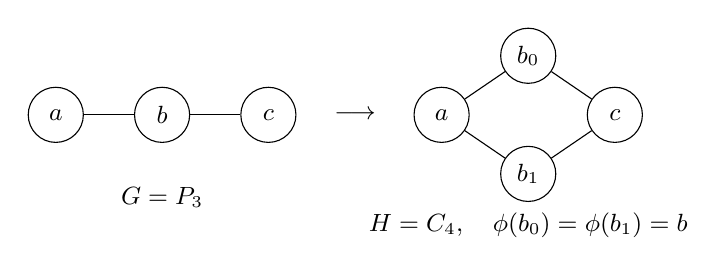
\begin{tikzpicture}[every node/.style={font=\small},
  vertex/.style={circle,draw,fill=white,minimum size=7mm,inner sep=1pt}]
\node[vertex] (a) at (0,0) {$a$};
\node[vertex] (b) at (1.35,0) {$b$};
\node[vertex] (c) at (2.7,0) {$c$};
\draw (a)--(b)--(c);
\node at (1.35,-1.05) {$G=P_3$};
\node at (3.8,0) {$\longrightarrow$};
\node[vertex] (aa) at (4.9,0) {$a$};
\node[vertex] (b0) at (6,0.75) {$b_0$};
\node[vertex] (cc) at (7.1,0) {$c$};
\node[vertex] (b1) at (6,-0.75) {$b_1$};
\draw (aa)--(b0)--(cc)--(b1)--(aa);
\node at (6,-1.4) {$H=C_4,\quad\phi(b_0)=\phi(b_1)=b$};
\end{tikzpicture}
\caption{A faithful expansion of $P_3$ into $C_4$. The two vertices
$b_0,b_1$ share the observable label $b$; the labels $a,c$ each have one
preimage. The projected walk has exactly the transition law on the path.}
\label{fig:path-cycle}
\end{figure}

From $a$ or $c$, the next observed label is always $b$. From either copy of
$b$, the next label is $a$ or $c$ with probability $1/2$ each. An observer
restricted to these labels cannot distinguish the trajectory laws at any
horizon, even though one graph is a tree and the other has a cycle. An
observer who can recognize individual microscopic vertices can distinguish
them: a walk begun at $b$ in $P_3$ returns to that very vertex in two steps
with probability $1$, whereas a walk begun at $b_0$ in $C_4$ returns to
$b_0$ in two steps with probability $1/2$.

\begin{corollary}[Hidden cycles in an optimal expansion]
For every vertex-minimizing expansion,
\[
 \beta(H)=2\beta(G)+\alpha(G)-1.
\]
In particular, if $G$ is a tree, an optimal expansion has exactly
$\alpha(G)-1$ independent cycles.
\end{corollary}
\begin{proof}
Both graphs are connected, and optimality gives
$|\E(H)|=2|\E(G)|$ and $|\V(H)|=2|\V(G)|-\alpha(G)$.
Substitute these into $\beta(H)=|\E(H)|-|\V(H)|+1$.
\end{proof}

For a star with $r$ leaves, splitting its center produces $K_{2,r}$.
This uses only one additional vertex and creates $r-1$ independent cycles.

\subsection{Time-dependent replacement}

\begin{proposition}[Changing the graph between observations]\label{prop:dynamic}
Let every $H_t$ have a faithful projection $\phi_t$ onto the same base $G$.
At each tick, move the current hidden vertex into any vertex of $H_{t+1}$
with the same base label, then take one simple-random-walk step in $H_{t+1}$.
The observed label sequence is exactly a simple random walk on $G$.
The choice of $H_{t+1}$ and the relocation may depend on the past, provided
they occur before the fresh uniform neighbor draw.
\end{proposition}
\begin{proof}
Relocation preserves the current label. Conditional on the entire past,
the next label has distribution $P_G(u,\cdot)$ for every possible relocated
vertex over $u$, by~\eqref{eq:local}. Averaging over relocation and applying
the chain rule proves the claim.
\end{proof}

The relocation is between observed ticks; it is not counted as an additional
walk step. Retaining the current base label is sufficient for preserving the
observed transition law across each replacement.

\subsection{Nested strict expansions}

\begin{corollary}[Cost of nested strict expansions]\label{cor:history}
Suppose each map in
\[
 G_T\xrightarrow{\phi_T}G_{T-1}\longrightarrow\cdots
       \xrightarrow{\phi_1}G_0
\]
is a nontrivial faithful expansion. Then the composite is faithful, and
\[
 |\E(G_T)|=\left(\prod_{t=1}^T D_t\right)|\E(G_0)|
       \ge2^T|\E(G_0)|.
\]
Thus an edge budget $M\ge|\E(G_0)|$ permits at most
$\lfloor\log_2(M/|\E(G_0)|)\rfloor$ successive strict expansions.
\end{corollary}
\begin{proof}
If $P_HC=CP_G$ and $P_GB=BP_F$, then $P_HCB=CBP_F$, proving composition.
Lemma~\ref{lem:degree} supplies an integer factor $D_t\ge2$ at each step;
multiplying the edge counts gives the result.
\end{proof}

The exponential cost concerns nested strict expansions. It does not apply
to histories that alternate expansion and contraction, to relabelings, or
to the arbitrary common-base replacements of Proposition~\ref{prop:dynamic}.

\section{Weighted expansions and scope}\label{sec:weights}

For a graph with positive edge weights $w_{xy}=w_{yx}$, the weighted walk
chooses $y$ from $x$ with probability $w_{xy}/\sum_z w_{xz}$. Allowing such
weights changes the minimum expansion cost.

\begin{proposition}[Minimum order with adjustable weights]
For every unweighted base graph $G$ in the main theorem, the smallest
nontrivial faithful expansion allowing positive edge weights has
$|\V(G)|+1$ vertices.
\end{proposition}
\begin{proof}
Surjectivity and nontriviality require at least one additional vertex.
Choose a vertex $v$ and replace it by two copies. Replace each edge $vu$
by two edges of weight $1/2$, one from each copy to $u$, and give every
other edge weight $1$. From $u$, the total weight toward label $v$ remains
$1$. From either copy of $v$, all original neighboring labels remain
equiprobable. All other transition probabilities are unchanged. The graph
is connected and the expansion is faithful, proving attainment.
\end{proof}

In particular, the vertex-cover bound depends on the unit-weight restriction.
Simplicity is also used essentially when bounding the number of edges
between singleton fibers in the proof of Theorem~\ref{thm:main}.

Likewise the observation restriction matters. The theorem preserves the
discrete-time trajectory of the original labels, not the microscopic
topology, individual-vertex return events, or a continuous-time walk with
unit rate on every edge.

\section{Computational verification}\label{sec:checks}

The accompanying program \texttt{verify\_random\_walk\_refinements.py}, run
with Python 3.13.7 and NetworkX 3.6.1, uses exact integer and rational
arithmetic. Its saved output is \texttt{verification\_results.json}.
\begin{table}[htbp]
\centering
\small
\caption{Exact finite checks of the extremal bounds and the classification.}
\label{tab:checks}
\begin{tabularx}{\textwidth}{@{}Xr@{}}
\toprule
Check & Count\\
\midrule
Connected base graphs, orders 2--7; optimal construction checked & 995\\
Source partitions with 2 through $n-1$ blocks, orders 2--7 & 770,021\\
Faithful nontrivial partitions found & 201\\
Vertex-bound equality cases among them & 37\\
Minimum covers used for classification checks, orders 2--5 & 71\\
Matching sign assignments checked by label-preserving isomorphism & 543\\
Counterexamples to the stated bounds or classification & 0\\
\bottomrule
\end{tabularx}
\end{table}

The exhaustive source check examines every set partition of every connected
Graph Atlas graph of orders 2--7, up to isomorphism of the source. This covers
every surjection up to renaming quotient labels. It derives the quotient
directly from the source and tests the one-step transition probabilities;
it does not restrict candidates to the proposed construction. For the path,
triangle, and four-leaf star examples, complete projected trajectory laws
were compared from every starting vertex through eight steps. Five nested
expansions from a single edge produced edge counts $1,2,4,8,16,32$, and the
composite projections were also checked. These finite checks supplement the
proofs; they do not replace them or constitute a formal proof-assistant
verification. Table~\ref{tab:checks} records the resulting counts.

\paragraph{Reproducibility.}
The verification script and its JSON output accompany the manuscript.
Executing \texttt{python3 verify\_random\_walk\_refinements.py} regenerates
all reported counts using NetworkX. The program uses integer comparisons
for one-step transition identities and rational arithmetic for trajectory
probabilities; no numerical tolerances enter the tests.

\begin{thebibliography}{9}
\bibitem{BN}
M. Baker and S. Norine,
\emph{Harmonic morphisms and hyperelliptic graphs},
International Mathematics Research Notices 2009, no.~15, 2914--2955.
\href{https://arxiv.org/abs/0707.1309}{arXiv:0707.1309}.
The lemma numbers cited above refer to the arXiv text.

\bibitem{GT}
B. C. Geiger and C. Temmel,
\emph{Lumpings of Markov chains, entropy rate preservation, and higher-order
lumpability},
\href{https://arxiv.org/abs/1212.4375}{arXiv:1212.4375}.
\end{thebibliography}

\end{document}
